% vim: set textwidth=78 autoindent:

\section{QGIS Plugins}\label{sec:plugins}\index{plugins}

% when the revision of a section has been finalized, 
% comment out the following line:
\updatedisclaimer

QGIS has been designed with a plugin architecture.
This allows new features/functions to be easily added to the application.
Many of the features in QGIS are actually implemented as \textbf{core} or \textbf{external} plugins.\index{plugins!types} 

\begin{itemize}
\item \textbf{Core Plugins} are maintained by the QGIS Development Team and are automatically part of every QGIS distribution.
More information about core plugins are provided in Section \ref{sec:core_plugins}.
\item \textbf{External Plugins} are currently all written in Python.
They are stored in external svn repositories and maintained by the individual author.
They can be added to QGIS using the core plugin called \filename{Fetch Python Plugins...}.
More information about external plugins are provided in Section \ref{sec:external_plugins}.
\end{itemize}

\subsection{Managing Plugins}\label{sec:managing_plugins}
\index{plugins!managing} 

Managing plugins in general means loading or unloading them using the \filename{Plugin Manager} and the \filename{Plugin installer} plugin. 

\subsubsection{Loading a QGIS Core Plugin}\label{sec:load_core_plugin} 

Loading a QGIS Core Plugin is provided in the main menu \mainmenuopt{Plugins} > \dropmenuopttwo{plugin_installer}{Manage Plugins...}.\index{plugins!manager}

\begin{figure}[ht]
   \begin{center}
   \caption{Plugin Manager \nixcaption}\label{fig:pluginmanager}\smallskip
   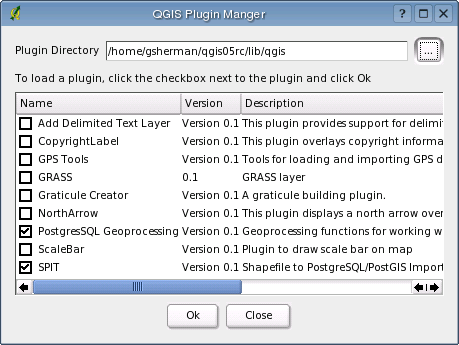
\includegraphics[clip=true, width=9cm]{pluginmanager}
\end{center}
\end{figure}

The Plugin Manager lists all the available plugins and their status (loaded or unloaded).
All available means all core plugins and all external plugins you added using \filename{Plugin Installer} plugin (see Section \ref{sec:external_plugins}). 
Figure \ref{fig:pluginmanager} shows the Plugin Manager dialog.
Loaded plugins are "remembered" when you exit the application and restored the next time you run QGIS.

Typically all QGIS core plugins are installed in the same location on your computer.
This location is shown in the Plugin Directory text field.
You can tell QGIS to load plugins from another location by specifying a different directory.

\begin{Tip}\caption{\textsc{Crashing Plugins}}\index{crashes}
\qgistip{If you find that QGIS crashes on startup, a plugin may be at fault.
You can stop all plugins from loading by editing your stored settings file (see \ref{subsec:gui_options} for location).
Locate the plugins settings and change all the plugin values to false to prevent them from loading.
\nix {For example, to prevent the Delimited text plugin from loading, the entry in \$HOME/.config/QuantumGIS/qgis.conf on Linux should look like this:\usertext{Add Delimited Text Layer=false}.}
\normalfont 
Do this for each plugin in the [Plugins] section.
You can then start QGIS and add the plugins one at a time from the Plugin Manger to determine which is causing the problem.}
\end{Tip} 

\subsubsection{Loading an external QGIS Plugin}\label{sec:load_external_plugin} 

To be able to integrate external plugins into QGIS you first need to load the \filename{Plugin Installer} plugin as desribed in Section \ref{sec:load_core_plugin}.
Then you can load external QGIS python plugin in two steps: 

\begin{enumerate}
\item Download an external plugin from a repository using the \filename{Plugin Installer}.
The new external plugin will be integrated into the list of available plugins in the \filename{Plugin Manager}.
\item Load the plugin using the \filename{Plugin Manager}.
\end{enumerate}

\begin{figure}[ht]
   \begin{center}
   \caption{Installing external python plugins \nixcaption}
\label{fig:plugininstaller}\smallskip
   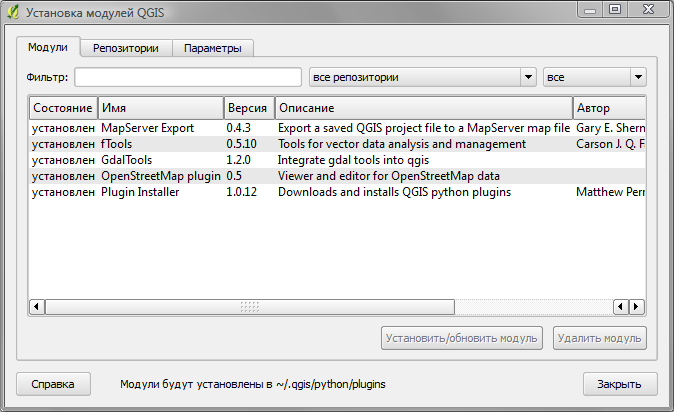
\includegraphics[clip=true, width=9cm]{plugininstaller}
\end{center}
\end{figure}

\subsection{Data Providers}\index{data providers}

Data Providers are "special" plugins that provides access to a data store.
By default, QGIS supports PostGIS layers and disk-based data stores supported by the GDAL/OGR library (Appendix \ref{appdx_ogr}).
A Data Provider plugin extends the ability of QGIS to use other data sources.

Data Provider plugins are registered automatically by QGIS at startup.
They are not managed by the Plugin Manager but are used behind the scenes when a corresponding data type is added as a layer in QGIS.
